
\renewcommand\appendixpagename{Appendix}
\begin{appendices}
\chapter{Data Clump Type Context}
\label{app:data_clump_format}
An example of the data clump type context can be seen in listing \ref{lst:data_clump_type_context_example}. Only a subset of the format will be discussed here for space reasons.

  \begin{figure} [htbp!]
			\lstinputlisting
			[caption={Example of Data Clump Type Context},
			label={lst:data_clump_type_context_example},
			captionpos=b,language=java, basicstyle=\footnotesize, tabsize=2, showstringspaces=false,  numbers=left]
			{figures/chapter2/data_clump_type_context_example.json}
		\end{figure}

The format consists of three layers. In the outer layer left out here, general project information is defined: The programming language or the project's location. Also the number of methods, classes, and the number of detected data clumps can be obtained in this general part. 

In the next layer, each detected data clump is mapped with a unique key (l. 4).

The detected data clumps are described as a link between two files. These files might be identical if the data clumps are located in the same file. Here, one must differentiate between the \enquote{from-part}, and the \enquote{to-part} representing the two nodes in the data clump graph. For instance, \enquote{from\_file\_path} indicates the location of one part of the data clump, while \enquote{to\_file\_path} provides the path to the opposite end. 

A similar principle is applied to the classes in which a data clump is located. Because a class name might not be unique, not only the names of the two classes but also unique identifiers of those classes are provided (l. 9-10 and 14-15).

The information about the methods of the data clump (l. 11, 12, 16, 17) is optional. If one part of the data clump is a field-to-field data clump, no method is involved, so the respective part would be \textit{null}.

The field \enquote{probability} can be used by probabilistic data clump detection tools to indicate the probability that the detected data clump is indeed a data clump. For purposes of this master's thesis, it will be ignored. 

In lines 19-42, each variable that is part of the data clump is described. In this example, only one variable is listed, although for a data clump there must be at least three variables. As for the data clump itself, the individual variables are separated into a \enquote{from-part} and a \enquote{to-part}. The former is implicitly defined (l.~20-25, 38-42), while the latter has a specifically named sub object \enquote{to\_variable} (l. 27-37). For each variable, the name (l. 22 and l. 28)) and the data type (l.~23 and l. 29) are provided. As for the general data clump, a probability is given whether the variable is indeed part of a data clump (l. 24). As mentioned above, this information will be ignored.  Additionally, modifiers like \enquote{private}, \enquote{final} etc. are also stored. 

In order to find the variable in the source code, detailed location information is needed. Parts of the location information are, the line number (l.~32 and l.~39) and the column number (l.~33 and l.~40). To avoid any ambiguity, the end position of the variable is saved, too. All numbers are one-index-based, meaning that the first line is one and the first column is also one. 


\chapter{Pull Request Text} \label{app:pr_text}


Title: \textbf{ Refactored data clumps with the help of LLMs (research project)}


Hello maintainers,

I am conducting a master's thesis project focused on enhancing code quality through automated refactoring of data clumps, assisted by Large Language Models (LLMs).\newline


\textbf{Data Clump Definition}
\newline

A data clump exists if
\begin{enumerate}
    \item  two methods (in the same or in different classes) have at least 3 common parameters and one of those methods does not override the other,  or
    \item  At least three fields in a class are common with the parameters of a method (in the same or in a different class), or
    \item  Two different classes have at least three common fields
\end{enumerate}

See also the following UML diagram as an example
\begin{figure}[htpb!]
    \centering
    \includesvg[width=0.75\columnwidth]{figures/appendix/data_clump_explained.svg}
    \caption{Example Data Clump}
    \label{fig:enter-label}
\end{figure}
    



I believe these refactoring can contribute to the project by reducing complexity and enhancing readability of your source code.

Pursuant to the EU AI Act, I fully disclose the use of LLMs in generating these refactorings, emphasizing that all changes have undergone human review for quality assurance. 


Even if you decide not to integrate my changes to your codebase (which is perfectly fine), I ask you to fill out a feedback survey, which will be scientifically evaluated to determine the acceptance of AI-supported refactorings. You can find the feedback survey under \url{https://campus.lamapoll.de/Data-clump-refactoring/en}


Thank you for considering my contribution. I look forward to your feedback. If you have any other questions or comments, feel free to write a comment, or email me under tschoemaker@uni-osnabrueck.de.
\newline

Best regards,\newline
Timo Schoemaker \newline
Department of Computer Science \newline
University of Osnabrück \newline


\chapter{Survey for experiment 1}\label{app:pr_survey}

For this master's thesis, the survey platform \textit{LamaPoll} \cite{lamapoll} was used.  The respondents should address the following statements:
\begin{enumerate}
\item Data clumps are a code smell that should be fixed.
\item Using LLMs in software development can be helpful to improve code quality.
\item The proposed refactoring maintains or improves the quality of the code.
\item The proposed refactoring has  adequately identified and preserved the original functionality and intent of the code.
\item The name of the new extracted class(es), fields and methods are well-chosen.
 \item The location of the extracted class(es) are well-chosen.
 \item For how long have you been contributing to this project?
\item For how long have you been a developer in Java ? 
\item Please input the URL of the GitHub project from where you got to this survey.

\end{enumerate}


The statements 7--9 are actually questions that do not use the Likert scale. Question 7 attempts to assess the experience of the developer about this project. Question 8 similarly is aimed to obtain the programming experience of the respondent in the Java language.

The purpose of question 9 is to create a connection between the survey and the pull request of the project as the survey platform does not allow such a link easily.

\begin{table}[ht!]
    \centering
    \begin{tabular}{m{5cm}|m{1cm}}
         Altitude & Likert-Score  \\\hline
        Strongly Disagree & 0.0\\\hline
        Disagree & 1.0 \\\hline
        Neutral & 2.0 \\\hline
        Agree & 3.0 \\\hline
    Strongly Agree & 4.0\\\hline
        
        
    \end{tabular}
    \caption{Likert Options}
    \label{tab:likert_options}
\end{table}

Table \ref{tab:likert_options} shows the options for each question and the associated Likert score.





\chapter{UML diagram of the tool} \label{app:uml_diagram}
Figure \ref{fig:uml_classes} depicts the most important classes of the tool in the scenario that data clumps are detected manually and the \ac{LLM} performs the refactoring. 

The following list describes the functionality of each class in this scenario:
\begin{description}
    \item [AbstractStepHandler] This abstract class is the foundation of each step handler. It provides the \textit{handle} method which executes a given step. It returns a new \textit{DataClumpRefactoringContext} based on the information obtained in this step and the previous context.
    \item [DataClumpRefactoringContext] This class represents the context. It is implemented as a linked list. 
    \item[SimpleCodeObtainingHandler] This step handler creates the first context which contains the project's location.

    \item [DataClumpDoctorStepHandler] This handler executes the \textit{DataClumpDoctor} and creates a context containing the detected data clumps
    \item [LanguageModelRefactorHandler] This handler uses the \ac{LLM} to perform the refactoring. A significant work is delegated to the \textit{LargeLanguageModelHandler}.

    \item [LargeLanguageModelHandler] This class converts the context and the configuration to create the static and dynamic resources. It then sends this data to the model and waits for its reply. 

    \item[AllFilesHandler] This handler loads the contents of all files containing data clumps and sends them to the model. 

    \item[LanguageModelTemplateResolver] This class deals with the static resources. It resolves the given instruction until it does not contain any templates.

    \item [AbstractLanguageModel] This class is an interface to an \ac{LLM}. It provides operations for queuing and sending messages to a model. 

    \item [ChatGPTInterface] This class is the implementation of the \textit{AbstractLanguageModel} for ChatGPT.
\end{description}
\begin{figure}
    \centering
    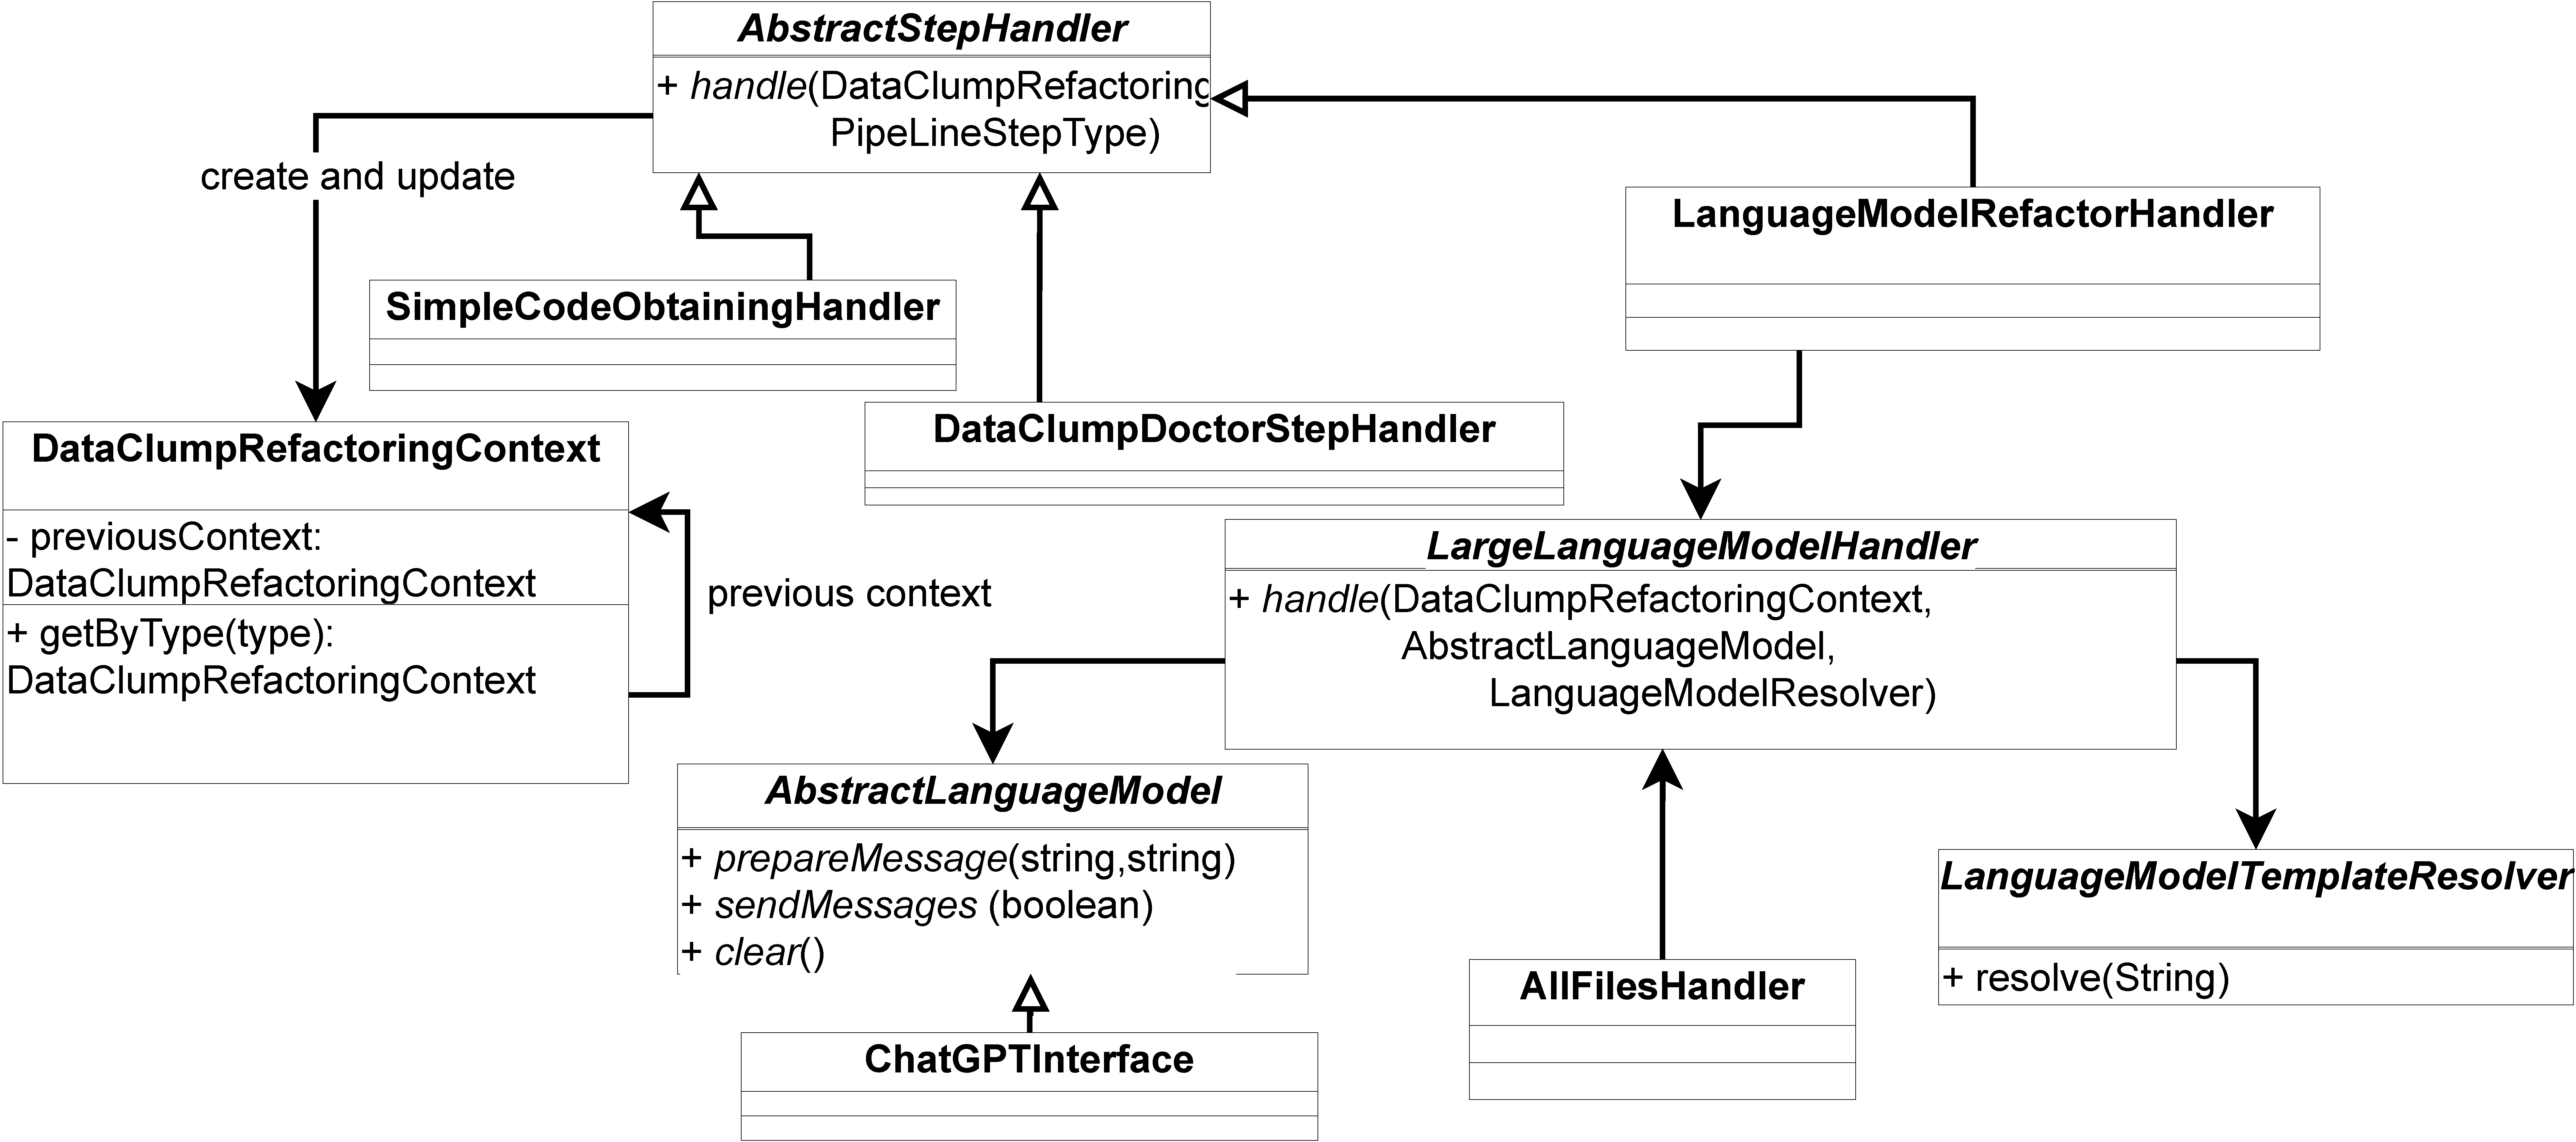
\includegraphics[ angle=90,
    width=0.6\columnwidth]{figures/appendix/class_diagram.drawio.pdf}
    \caption{UML Diagram: Important classes of the tool for refactoring with \ac{LLM}}
    \label{fig:uml_classes}
\end{figure}
\end{appendices}
	
